\section{Biểu đồ hoạt động}
\subsection{Đăng nhập}
\begin{center}
	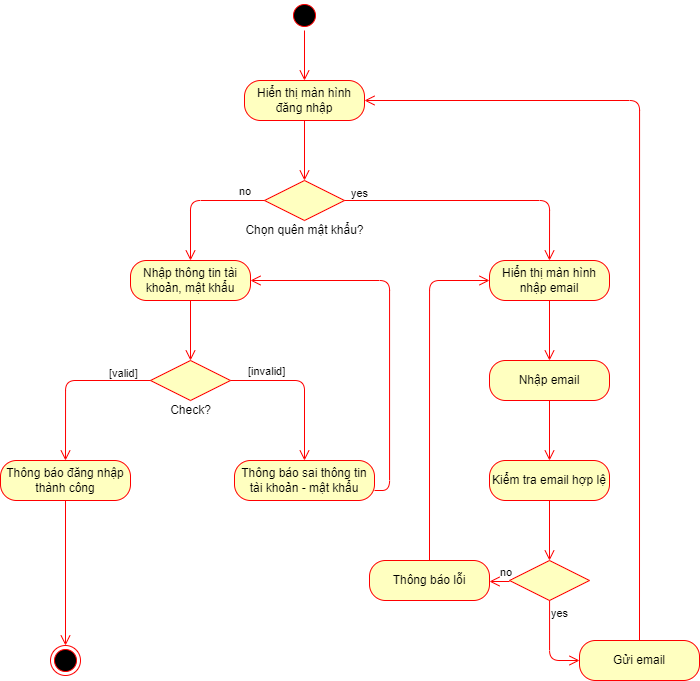
\includegraphics[width=1.1\textwidth]{../drawio/activity/login.png}
	\begin{figure}[h]
		\centering
		\caption{Biểu đồ đăng nhập}
	\end{figure}
\end{center}
\begin{tabular}{|l|l|}
	\hline
	\textbf{Các tác nhân}         & Admin, sinh viên, giảng viên, giáo vụ, trưởng phòng \\
	\hline
	\textbf{Mô tả}                & Đăng nhập                                           \\
	\hline
	\textbf{Kích hoạt}            & Người dùng nhấn vào nút "Đăng nhập" trên thanh menu \\
	\hline
	\textbf{Luồng chính}          & \makecell[l]{1. Chọn chức năng đăng nhập            \\ 2. Hiển thị màn hình đăng nhập \\ 3. Nhập tên đăng nhập và mật khẩu \\ 4. Hiển thị kiểm tra thông tin \\ 5. Nếu thành công chuyển tới giao diện chính \\ 6. Kết thúc} \\
	\hline
	\textbf{Các luồng thay thế}   & \makecell[l]{Mật khẩu không hợp lệ:                 \\ 1. Thông báo ra màn hình mật khẩu sai \\ 2. Quay lại bước 2 của luồng chính \\ Quên mật khẩu: \\ 1. Hiển thị màn hình nhập email \\ 2. Nhập và chọn chức năng quên mật khẩu \\ 3. Kiểm tra hợp lệ hệ thống gửi mail xác nhận \\ 4. Hiển thị thông báo thành công \\ 5. Kết thúc} \\
	\hline
	\textbf{Tiền điều kiện}       & Tài khoản trước đó đã được đăng ký                  \\
	\hline
	\textbf{Hậu điều kiện}        & Người dùng đăng nhập thành công                     \\
	\hline
	\textbf{Các yêu cầu đặc biệt} &                                                     \\
	\hline
\end{tabular}

\subsection{Đăng ký}
\begin{center}
	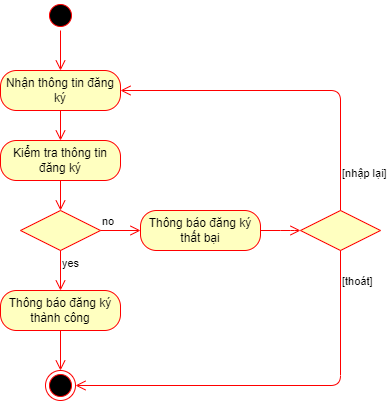
\includegraphics[width=1.1\textwidth]{../drawio/activity/logup.png}
	\begin{figure}[h]
		\centering
		\caption{Biểu đồ đăng ký}
	\end{figure}
\end{center}
\begin{tabular}{|l|p{0.8\textwidth}|}
	\hline
	\textbf{Các tác nhân}       & Admin, sinh viên, giảng viên                                        \\
	\hline
	\textbf{Mô tả}              & Đăng ký                                                             \\
	\hline
	\textbf{Kích hoạt}          & Người dùng nhấn vào nút "Đăng ký" trên thanh menu                   \\
	\hline
	\textbf{Luồn chính}         & \makecell[l]{Trường hợp bắt đầu khi người truy cập muốn đăng ký tài \\khoản mới: \\ 1. Chọn chức năng đăng ký \\ 2. Màn hình hiển thị form đăng ký \\ 3. Hệ thống nhận các thông tin, thực hiện validate \\ 4. Thông báo đăng ký thành công \\ 5. Kết thúc} \\
	\hline
	\textbf{Các luồng thay thế} & \makecell[l]{Đăng ký thất bại:                                      \\ - Thông tin đăng ký không hợp lệ \\ - Email đã được đăng ký} \\
	\hline
	\textbf{Tiền điều kiện}     & Người dùng trước đó đã đăng nhập                                    \\
	\hline
	\textbf{Hậu điều kiện}      & Người dùng đăng xuất thành công                                     \\
	\hline
	\textbf{Yêu cầu đặc biệt}   &                                                                     \\
	\hline
\end{tabular}

\subsection{Đăng xuất}
\begin{center}
	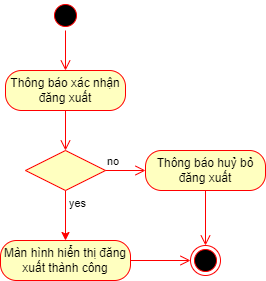
\includegraphics[width=.7\textwidth]{../drawio/activity/logout.png}
	\begin{figure}[h]
		\centering
		\caption{Biểu đồ đăng xuất}
	\end{figure}
\end{center}
\begin{tabular}{|l|l|}
	\hline
	\textbf{Các tác nhân}         & Admin, sinh viên, giảng viên, giáo vụ, trưởng phòng                              \\
	\hline
	\textbf{Mô tả}                & Đăng xuất                                                                        \\
	\hline
	\textbf{Kích hoạt}            & Người dùng nhấn vào nút "Đăng xuất" trên thanh menu                              \\
	\hline
	\textbf{Luồn chính}           & \makecell[l]{Trường hợp bắt đầu khi người truy cập muốn đăng xuất khỏi hệ thống: \\ 1. Chọn chức năng đăng xuất \\ 2. Màn hình hiển thị thông báo xác nhận muốn đăng xuất \\ 3. Thông báo đăng xuất thành công \\ 4. Kết thúc} \\
	\hline
	\textbf{Các luồng thay thế}   & Không có                                                                         \\
	\hline
	\textbf{Tiền điều kiện}       & Người dùng trước đó đã đăng nhập                                                 \\
	\hline
	\textbf{Hậu điều kiện}        & Người dùng đăng xuất thành công                                                  \\
	\hline
	\textbf{Các yêu cầu đặc biệt} &                                                                                  \\
	\hline
\end{tabular}

\subsection{Quên mật khẩu}
\begin{center}
	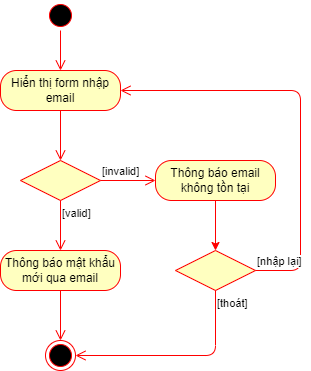
\includegraphics[width=.7\textwidth]{../drawio/activity/forgot_password.png}
	\begin{figure}[h]
		\centering
		\caption{Biểu đồ quên mật khẩu}
	\end{figure}
\end{center}
\begin{tabular}{|l|l|}
	\hline
	\textbf{Các tác nhân}         & Admin, sinh viên, giảng viên                            \\
	\hline
	\textbf{Mô tả}                & Quên mật khẩu                                           \\
	\hline
	\textbf{Kích hoạt}            & Người dùng nhấn vào nút "Quên mật khẩu" trên thanh menu \\
	\hline
	\textbf{Luồn chính}           & \makecell[l]{1. Người dùng chọn chức năng quên mật khẩu \\ 2. Hệ thống tiếp nhận thông tin email \\ 3. Hệ thống kiểm tra email \\ 4. Hệ thống thông báo mật khẩu mới được gửi qua email \\ 5. Kết thúc} \\
	\hline
	\textbf{Các luồng thay thế}   & \makecell[l]{Thông tin email không hợp lệ:              \\ 1. Thông báo thông tin email không đúng \\ 2. Trở lại màn hình nhập email \\ 3. Kết thúc} \\
	\hline
	\textbf{Tiền điều kiện}       & email trước đó đã được dùng để đăng ký tài khoản        \\
	\hline
	\textbf{Hậu điều kiện}        & mật khẩu mới của tài khoản email xác nhận               \\
	\hline
	\textbf{Các yêu cầu đặc biệt} &                                                         \\
	\hline
\end{tabular}

\subsection{Cập nhật thông tin}
\begin{center}
	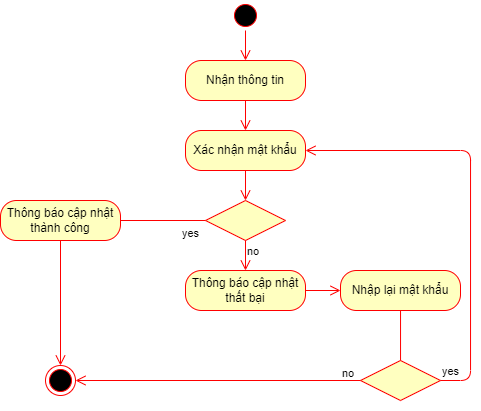
\includegraphics[width=1.1\textwidth]{../drawio/activity/updatedata.png}
	\begin{figure}[h]
		\centering
		\caption{Biểu đồ cập nhật thông tin}
	\end{figure}
\end{center}
\begin{tabular}{|l|l|}
	\hline
	\textbf{Các tác nhân}         & Admin, sinh viên, giảng viên                                                              \\
	\hline
	\textbf{Mô tả}                & Cập nhật thông tin cá nhân của người dùng, điểm của sinh viên, thông tin đồ án giảng viên \\
	\hline
	\textbf{Kích hoạt}            & Người dùng vào trang cá nhân và chọn chức năng "cập nhật thông tin"                       \\
	\hline
	\textbf{Luồn chính}           & \makecell[l]{1. Người dùng chọn chức năng cập nhật thông tin                              \\ 2. Hệ thống tiếp nhận thông tin cập nhật \\ 3. Hệ thống yêu cầu xác nhận mật khẩu \\ 4. Hệ thống kiểm tra mật khẩu \\ 5. Hệ thống thông báo cập nhật thành công \\ 6. Kết thúc} \\
	\hline
	\textbf{Các luồng thay thế}   & Không có                                                                                  \\
	\hline
	\textbf{Tiền điều kiện}       & người dùng đã đăng nhập                                                                   \\
	\hline
	\textbf{Hậu điều kiện}        & cập nhật thông tin thành công                                                             \\
	\hline
	\textbf{Các yêu cầu đặc biệt} &                                                                                           \\
	\hline
\end{tabular}

\subsection{Thống kê}
\begin{center}
	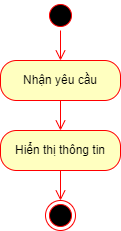
\includegraphics[width=.3\textwidth]{../drawio/activity/statistical.png}
	\begin{figure}[h]
		\centering
		\caption{Biểu đồ thống kê}
	\end{figure}
\end{center}
\begin{tabular}{|l|l|}
	\hline
	\textbf{Các tác nhân}         & Admin, giảng viên, giáo vụ, trưởng phòng                                                                                           \\
	\hline
	\textbf{Mô tả}                & Thống kê các thông tin: điểm CPA, số tín chỉ nợ, mức cảnh báo của các sinh viên; số lượng đăng ký đồ án; số lượng đăng ký thực tập \\
	\hline
	\textbf{Kích hoạt}            & Người dùng chọn chức năng thống kê trên hệ thống                                                                                   \\
	\hline
	\textbf{Luồn chính}           & \makecell[l]{1. Hệ thống tiếp nhận yêu cầu thống kê                                                                                \\ 2. Hệ thống lấy dữ liệu \\ 3. Hệ thống hiển thị biểu đồ thống kê \\ 4. Kết thúc} \\
	\hline
	\textbf{Các luồng thay thế}   & Không có                                                                                                                           \\
	\hline
	\textbf{Tiền điều kiện}       & Người dùng đã đăng nhập trước đó                                                                                                   \\
	\hline
	\textbf{Hậu điều kiện}        & Hiển thị biểu đồ thống kê chi tiết                                                                                                 \\
	\hline
	\textbf{Các yêu cầu đặc biệt} &                                                                                                                                    \\
	\hline
\end{tabular}

\subsection{Đăng ký đồ án}
\begin{center}
	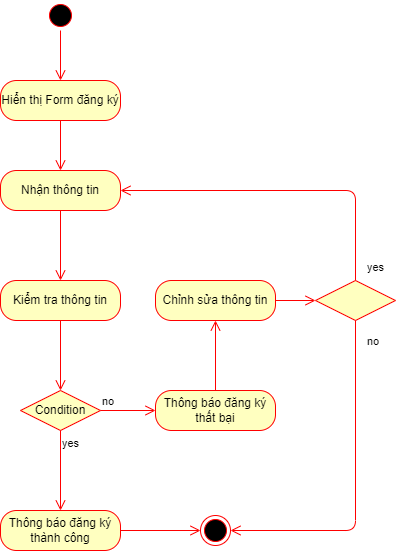
\includegraphics[width=.9\textwidth]{../drawio/activity/register_doan.png}
	\begin{figure}[h]
		\centering
		\caption{Biểu đồ đăng ký đồ án}
	\end{figure}
\end{center}
\begin{tabular}{|l|l|}
	\hline
	\textbf{Các tác nhân}         & Sinh viên                                                                                         \\
	\hline
	\textbf{Mô tả}                & Điền form thông tin đăng ký nhận đồ án                                                            \\
	\hline
	\textbf{Kích hoạt}            & Người dùng chọn chức năng đăng ký đồ án                                                           \\
	\hline
	\textbf{Luồn chính}           & \makecell[l]{Vào đầu mỗi kỳ học, admin mở chức năng đăng ký đồ án, sinh viên thực hiện điền form: \\ 1. Hệ thống hiển thị form nhập thông tin \\ 2. Hệ thống tiếp nhận thông tin \\ 3. Hệ thống kiểm tra thông tin \\ 4. Hệ thống trả về thông báo đăng ký thành công \\ 5. Kết thúc} \\
	\hline
	\textbf{Các luồng thay thế}   & không có                                                                                          \\
	\hline
	\textbf{Tiền điều kiện}       & Sinh viên đã đăng nhập tài khoản trước đó                                                         \\
	\hline
	\textbf{Hậu điều kiện}        &                                                                                                   \\
	\hline
	\textbf{Các yêu cầu đặc biệt} &                                                                                                   \\
	\hline
\end{tabular}

\subsection{Tạo CV}
\begin{center}
	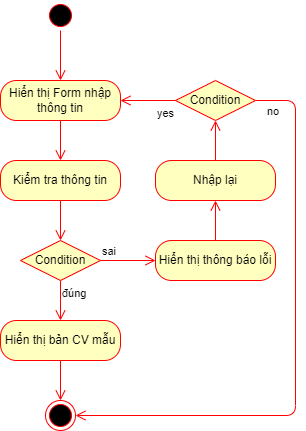
\includegraphics[width=.7\textwidth]{../drawio/activity/create_CV.png}
	\begin{figure}[h]
		\centering
		\caption{Biểu đồ tạo CV}
	\end{figure}
\end{center}
\begin{tabular}{|l|l|}
	\hline
	\textbf{Các tác nhân}         & Sinh viên                                             \\
	\hline
	\textbf{Mô tả}                & Thực hiện tạo CV cá nhân để đăng ký thực tập          \\
	\hline
	\textbf{Kích hoạt}            & Người dùng chọn chức năng "tạo CV"                    \\
	\hline
	\textbf{Luồn chính}           & \makecell[l]{1. Hệ thống hiển thị form nhập thông tin \\ 2. Hệ thống tiếp nhận thông tin \\ 3. Hệ thống kiểm tra thông tin \\ 4. Hệ thống trả về file CV \\ 5. Kết thúc} \\
	\hline
	\textbf{Các luồng thay thế}   & không có                                              \\
	\hline
	\textbf{Tiền điều kiện}       & Sinh viên đã thực hiện đăng nhập trước đó             \\
	\hline
	\textbf{Hậu điều kiện}        &                                                       \\
	\hline
	\textbf{Các yêu cầu đặc biệt} &                                                       \\
	\hline
\end{tabular}

\subsection{Đăng ký thực tập}
\begin{center}
	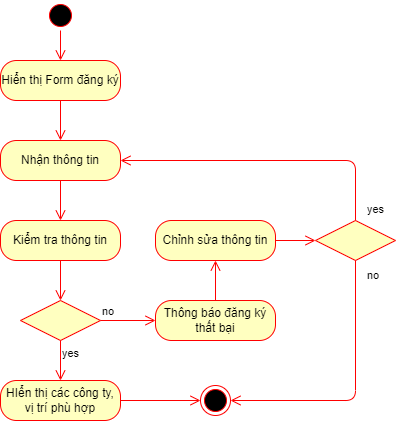
\includegraphics[width=.9\textwidth]{../drawio/activity/register_thuctap.png}
	\begin{figure}[h]
		\centering
		\caption{Biểu đồ đăng ký thực tập}
	\end{figure}
\end{center}
\begin{tabular}{|l|l|}
	\hline
	\textbf{Các tác nhân}         & Sinh viên                                             \\
	\hline
	\textbf{Mô tả}                & Sinh viên thực hiện đăng ký công ty, vị trí thực tập  \\
	\hline
	\textbf{Kích hoạt}            & Người dùng chọn chức năng "đăng ký thực tập"          \\
	\hline
	\textbf{Luồn chính}           & \makecell[l]{1. Hệ thống hiển thị form điền thông tin \\ 2. Hệ thống tiếp nhận thông tin \\ 3. Hệ thống lọc thông tin \\ 4. Hệ thống hiển thị các thông tin phù hợp \\ 5. Kết thúc} \\
	\hline
	\textbf{Các luồng thay thế}   & không có                                              \\
	\hline
	\textbf{Tiền điều kiện}       & Sinh viên đã đăng nhập trước đó                       \\
	\hline
	\textbf{Hậu điều kiện}        &                                                       \\
	\hline
	\textbf{Các yêu cầu đặc biệt} &                                                       \\
	\hline
\end{tabular}

\subsection{Tra cứu thông tin}
\begin{center}
	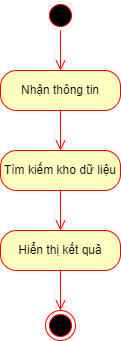
\includegraphics[width=.3\textwidth]{../drawio/activity/search_info.png}
	\begin{figure}[h]
		\centering
		\caption{Biểu đồ tìm kiếm}
	\end{figure}
\end{center}
\begin{tabular}{|l|l|}
	\hline
	\textbf{Các tác nhân}         & Sinh viên, giảng viên, giáo vụ, trưởng phòng, khách                     \\
	\hline
	\textbf{Mô tả}                & Tìm kiếm thông tin sinh viên, giảng viên, đề tài đồ án, vị trí thực tập \\
	\hline
	\textbf{Kích hoạt}            & Người dùng nhấn nút "tìm kiếm" trên thanh menu                          \\
	\hline
	\textbf{Luồn chính}           & \makecell[l]{1. Hệ thống tiếp nhận thông tin                            \\ 2. Hệ thống tìm kiếm trong cơ sở dữ liệu \\ 3. Hệ thống hiển thị kết quả \\ 4. Kết thúc} \\
	\hline
	\textbf{Các luồng thay thế}   & không có                                                                \\
	\hline
	\textbf{Tiền điều kiện}       & không có                                                                \\
	\hline
	\textbf{Hậu điều kiện}        & không có                                                                \\
	\hline
	\textbf{Các yêu cầu đặc biệt} &                                                                         \\
	\hline
\end{tabular}
